\documentclass[11pt, letterpaper]{amsart}

\usepackage[latin1]{inputenc}
\usepackage[USenglish,british,american,australian,english]{babel}
\usepackage{amsmath,amssymb,amsfonts,amsthm}
\usepackage{graphicx}
\usepackage[T1]{fontenc}

\usepackage{braket}
\usepackage{mathrsfs}
\usepackage{subfigure}
\usepackage{listings}
\usepackage{lettrine}
\usepackage{epigraph}
\usepackage{wrapfig}
\usepackage{bm}
\usepackage[font={scriptsize,sl},format=hang,labelfont={sf,bf}]{caption}
\usepackage[final]{hyperref}
\usepackage{cite}
\usepackage[margin=1in,letterpaper]{geometry}
\usepackage{url}
\usepackage{ctable}

\graphicspath{{figures/}}

\newcommand\norm[1]{\left\lVert#1\right\rVert}

\hyphenpenalty=20000
\tolerance=10000
\hbadness=10000

\title{Simulation of Fluid Flow in a Tesla Valve.}
\author{Hatef Khadivinassab, Daniele Rizzi}
\date{July 2, 2020}

\begin{document}
\maketitle

%-----------------------------------------------------------------------------------------------------------------
\section{Project aim}
In our project we have analysed the diodicity of two Tesla microvalve designs with a 3D CFD simulation using the open source computing platform FEniCS.
The basic design of this valve consists of channel that is split in a Y junction that re-enters in a T channel\footnote{Source: \url{https://en.wikipedia.org/wiki/Microvalve}}, as it can be seen in \ref{fig:designA-v3-vel} and \ref{fig:designB-v3-vel}.
Such a valve, is structured to have a higher pressure drop for the flow in one direction (reverse) than the other (forward). The efficiency of the valve is expressed in terms of the diodicity $D_i$, defined as the ratio of pressure drops for identical flow rates

\begin{equation}
	D_i = \left({\frac {\Delta p_{r}}{\Delta p_{f}}}\right)_{Q}
	\label{eq:diodicity}
\end{equation}

\noindent where $\Delta p_{r}$ is the reverse flow pressure drop and $\Delta p_{f}$ the forward flow pressure drop for flow rate.

%-----------------------------------------------------------------------------------------------------------------
\section{Results}
The velocity profiles at steady state for a type of Tesla microvalve are shown in figures \ref{fig:designA-v3-vel}.
\newline
As it can be seen by comparing the velocity profiles of forward (figures on the left) and reverse flow (figures on the right), in all the simulated cases the velocity fields of forward and reverse flow are significantly different.
\newline
In our project we studied how the diodicity of the Tesla Valve changes with fluid inlet velocity and the geometry of the Tesla Valve as reported in table \ref{table:diodicity}.
\newline
As it can be seen by comparing the results at the three different inlet velocities taken into account in the simulation, the diodicity of the same Tesla microvalve increases with the inlet velocity. In the case of reverse flow, the flow is splitted in the side and main channel when reaching the Y-junction. 
When the inlet velocity increases ($1.5 m/s$ and $5.0 m/s$), an higher volume of fluid is drained into the side channel with respect to the main channel; in this condition, when the side flow is re-injected in the main channel, it opposes to the main flow with the effect of increasing the pressure drop. By definition of the diodicity \ref{eq:diodicity}, the increase in the reverse pressure drop causes an increase in the diodicity.
\newline
The geometry of the Tesla microvalve has an important effect on the diodicity too. As one can imagine, when the angle of the T-junction is increased, the side flow is expected to be more opposed to the main flow causing higher reverse pressure drops in Design B with respect to Design A. However, as reported in table \ref{table:diodicity}, we found that the diodicity values of Design A and B are the same in the case of inlet velocity $0.3 m/s$, and at inlet velocities $1.5 m/s$ and $5.0 m/s$ they are even lower in the case of Design B with respect to Design A. This unexpected result could be explained by the presence of flaws in the model implemented in the simulation, which does not take into account capillarity, a physical effect important when studying the behavior of fluids in micro channels, or flaws in the design that should be studied deeper by evaluating the diodicity in other Tesla valve designs.

\begin{table}[!ht]
	\centering
	\caption{Diodicity values for designs A and B at different inlet velocities.}
	\begin{tabular}{c c c c}
		name     & $U=0.3m/s$ & $U=1.5m/s$ & $U=5m/s$ \\
		\hline \hline
		Design A & 1.0061 & 1.2807     & 1.3796      \\
		\hline
		Design B & 1.0079 & 1.1429     & 1.3440      \\
		\specialrule{.1em}{.05em}{.05em}
	\end{tabular}
	\label{table:diodicity}
\end{table}


\begin{figure}[!ht]
	\centering
	\subfigure[\label{fig:designA-v3}]
	{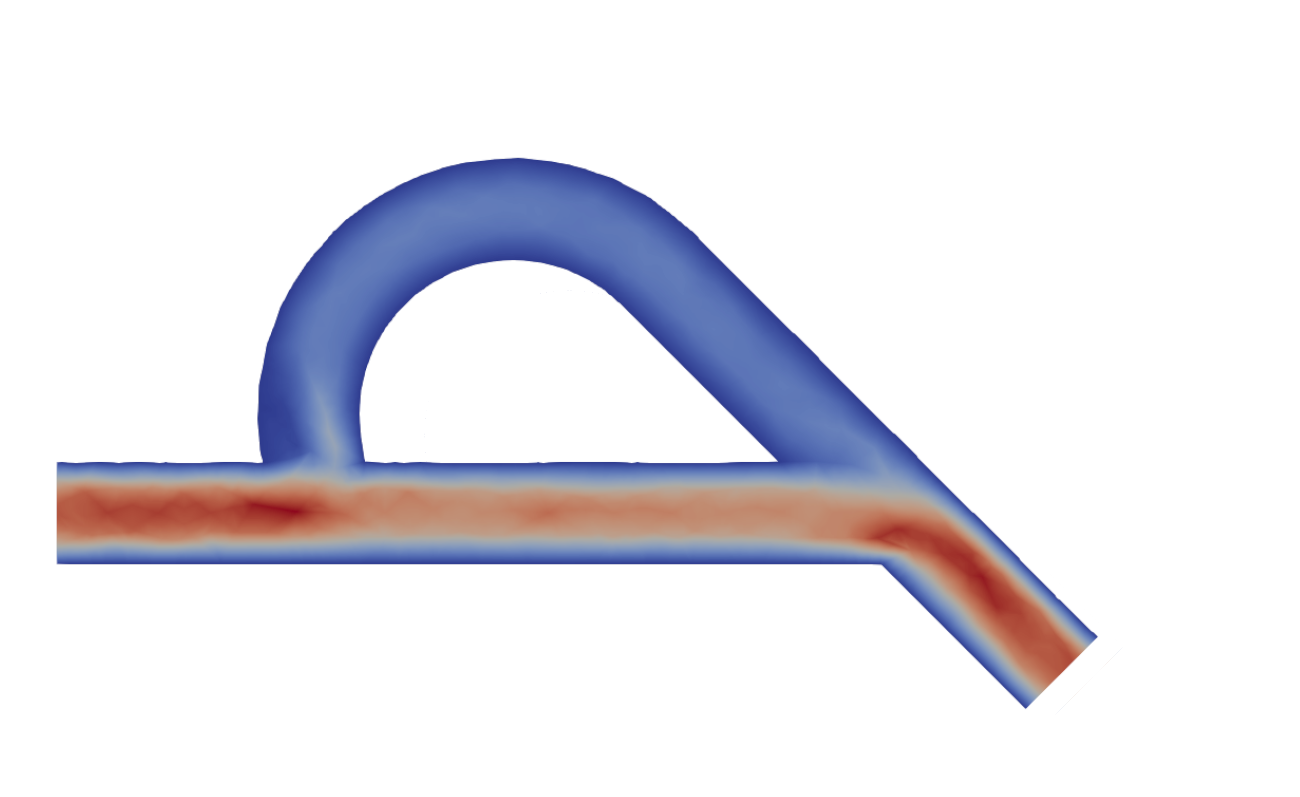
\includegraphics[angle=0,width=0.45\linewidth]{designA-v3.png}}
	\subfigure[\label{fig:designA-reverse-v3}]
	{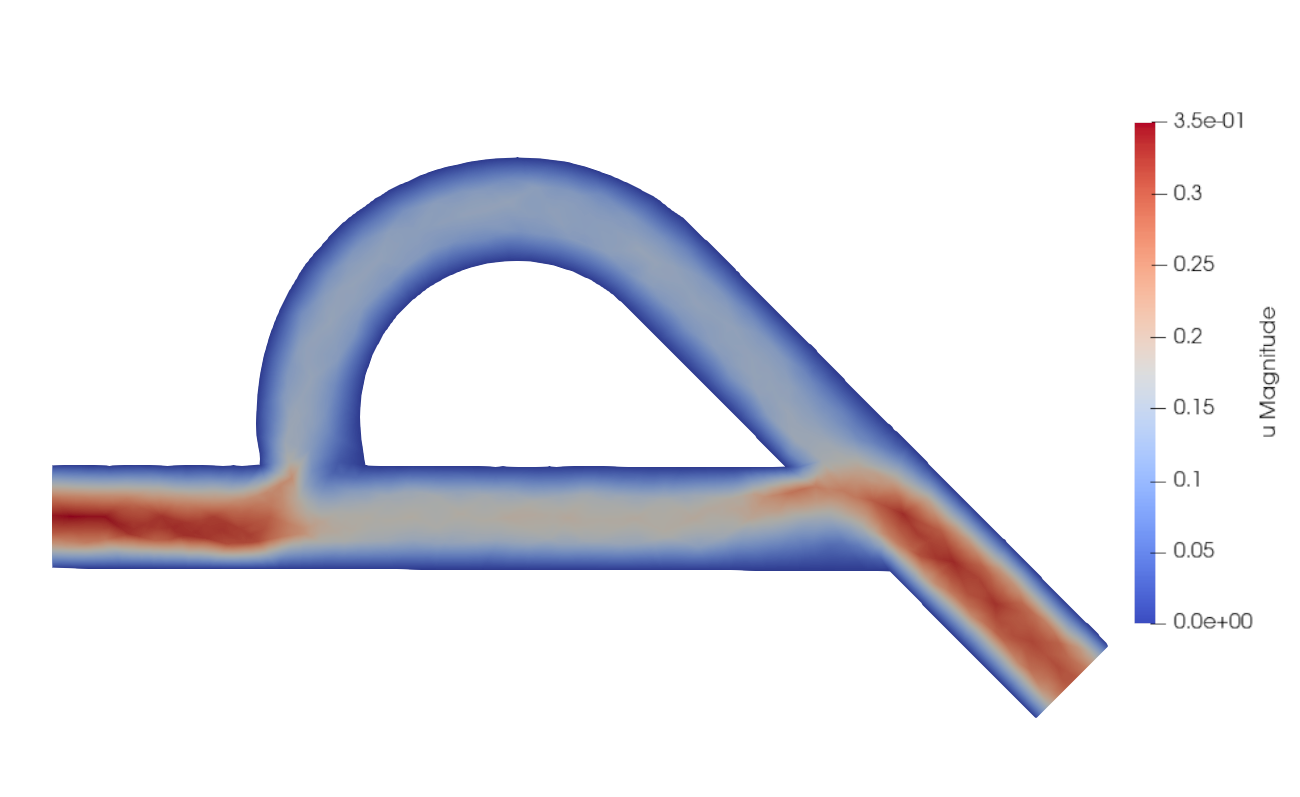
\includegraphics[angle=0,width=0.45\linewidth]{designA-reverse-v3.png}}
	\caption{Velocity results for design A with $U=0.3 m/s$ with forward flow (a) and reverse flow (b).}
	\label{fig:designA-v3-vel}
\end{figure}

\begin{figure}[!ht]
	\centering
	\subfigure[\label{fig:designB-v3}]
	{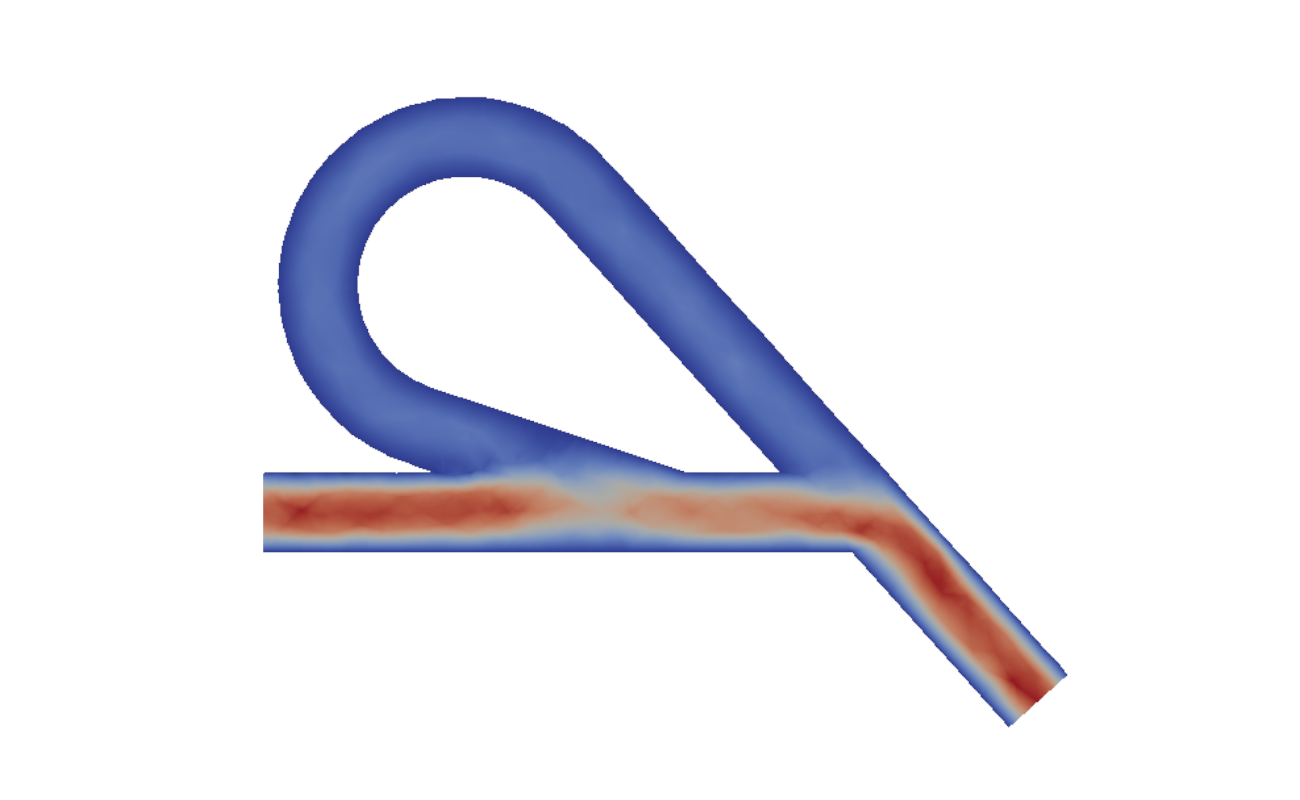
\includegraphics[angle=0,width=0.49\linewidth]{designB-v3.png}}
	\subfigure[\label{fig:designB-reverse-v3}]
	{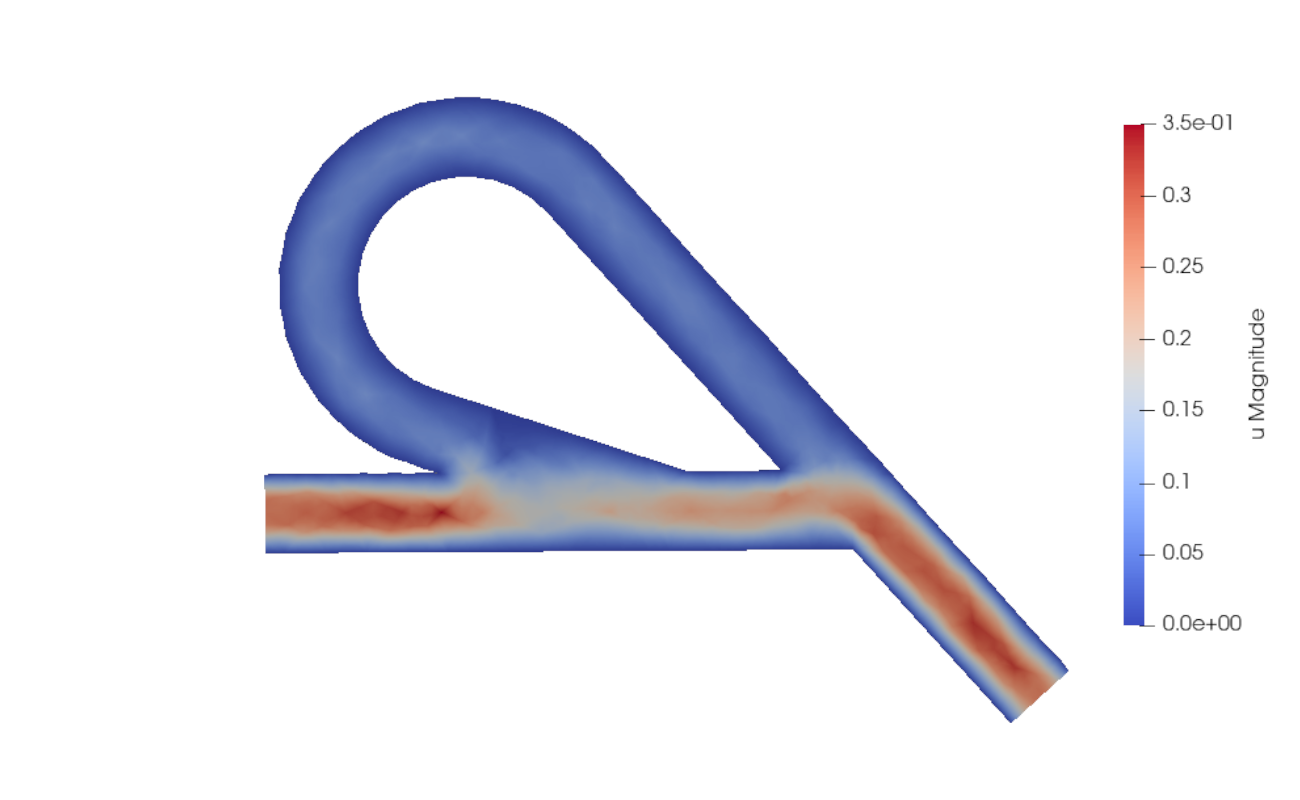
\includegraphics[angle=0,width=0.5\linewidth]{designB-reverse-v3.png}}
	\caption{Velocity results for design B with $U=0.3 m/s$ with forward flow (a) and reverse flow (b).}
	\label{fig:designB-v3-vel}
\end{figure}

\end{document}

